\section{moeo\-Additive\-Binary\-Epsilon\-Indicator$<$ EOFitness $>$ Class Template Reference}
\label{classmoeoAdditiveBinaryEpsilonIndicator}\index{moeoAdditiveBinaryEpsilonIndicator@{moeoAdditiveBinaryEpsilonIndicator}}
Functor Additive binary epsilon indicator for {\bf eo\-Pareto\-Fitness}.  


{\tt \#include $<$moeo\-Binary\-Quality\-Indicator.h$>$}

Inheritance diagram for moeo\-Additive\-Binary\-Epsilon\-Indicator$<$ EOFitness $>$::\begin{figure}[H]
\begin{center}
\leavevmode
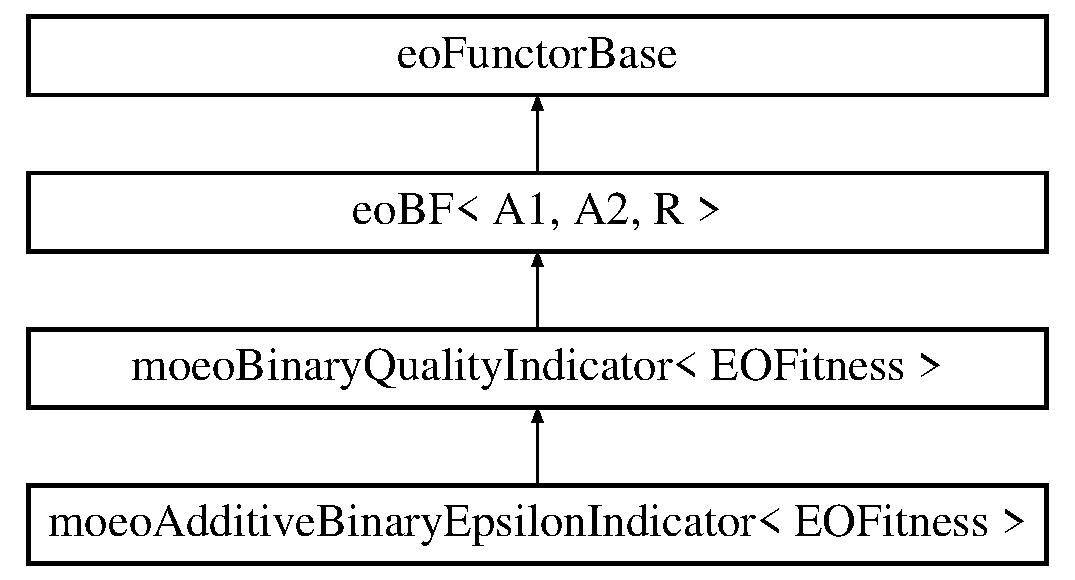
\includegraphics[height=4cm]{classmoeoAdditiveBinaryEpsilonIndicator}
\end{center}
\end{figure}
\subsection*{Public Member Functions}
\begin{CompactItemize}
\item 
{\bf moeo\-Additive\-Binary\-Epsilon\-Indicator} ()\label{classmoeoAdditiveBinaryEpsilonIndicator_d26af04a8276654998b4425f97963c47}

\begin{CompactList}\small\item\em constructor \item\end{CompactList}\item 
double {\bf operator()} (const EOFitness \&\_\-fitness\_\-eo1, const EOFitness \&\_\-fitness\_\-eo2)
\begin{CompactList}\small\item\em computation of the maximum epsilon value by which individual \_\-eo1 must be decreased in all objectives such that individual \_\-eo2 is weakly dominated (do not forget to set the bounds before the call of this function) \item\end{CompactList}\end{CompactItemize}
\subsection*{Private Types}
\begin{CompactItemize}
\item 
typedef EOFitness::fitness\_\-traits {\bf traits}\label{classmoeoAdditiveBinaryEpsilonIndicator_43e2945121a3e77683d935bc72399992}

\begin{CompactList}\small\item\em fitness traits \item\end{CompactList}\end{CompactItemize}
\subsection*{Private Member Functions}
\begin{CompactItemize}
\item 
double {\bf epsilon\-Value} (const EOFitness \&\_\-fitness\_\-eo1, const EOFitness \&\_\-fitness\_\-eo2, const unsigned \_\-i\-Obj)
\begin{CompactList}\small\item\em computation of the epsilon value by which individual \_\-eo1 must be decreased in the objective \_\-i\-Obj such that individual \_\-eo2 is weakly dominated \item\end{CompactList}\end{CompactItemize}


\subsection{Detailed Description}
\subsubsection*{template$<$class EOFitness$>$ class moeo\-Additive\-Binary\-Epsilon\-Indicator$<$ EOFitness $>$}

Functor Additive binary epsilon indicator for {\bf eo\-Pareto\-Fitness}. 



Definition at line 115 of file moeo\-Binary\-Quality\-Indicator.h.

\subsection{Member Function Documentation}
\index{moeoAdditiveBinaryEpsilonIndicator@{moeo\-Additive\-Binary\-Epsilon\-Indicator}!operator()@{operator()}}
\index{operator()@{operator()}!moeoAdditiveBinaryEpsilonIndicator@{moeo\-Additive\-Binary\-Epsilon\-Indicator}}
\subsubsection{\setlength{\rightskip}{0pt plus 5cm}template$<$class EOFitness$>$ double {\bf moeo\-Additive\-Binary\-Epsilon\-Indicator}$<$ EOFitness $>$::operator() (const EOFitness \& {\em \_\-fitness\_\-eo1}, const EOFitness \& {\em \_\-fitness\_\-eo2})\hspace{0.3cm}{\tt  [inline]}}\label{classmoeoAdditiveBinaryEpsilonIndicator_177f9999db6c9fb95d5fbff5a157348c}


computation of the maximum epsilon value by which individual \_\-eo1 must be decreased in all objectives such that individual \_\-eo2 is weakly dominated (do not forget to set the bounds before the call of this function) 

\begin{Desc}
\item[Parameters:]
\begin{description}
\item[{\em EOFitness}]\& \_\-fitness\_\-eo1 the fitness of the first individual \item[{\em EOFitness}]\& \_\-fitness\_\-eo2 the fitness of the second individual \end{description}
\end{Desc}


Definition at line 138 of file moeo\-Binary\-Quality\-Indicator.h.

References moeo\-Additive\-Binary\-Epsilon\-Indicator$<$ EOFitness $>$::epsilon\-Value().\index{moeoAdditiveBinaryEpsilonIndicator@{moeo\-Additive\-Binary\-Epsilon\-Indicator}!epsilonValue@{epsilonValue}}
\index{epsilonValue@{epsilonValue}!moeoAdditiveBinaryEpsilonIndicator@{moeo\-Additive\-Binary\-Epsilon\-Indicator}}
\subsubsection{\setlength{\rightskip}{0pt plus 5cm}template$<$class EOFitness$>$ double {\bf moeo\-Additive\-Binary\-Epsilon\-Indicator}$<$ EOFitness $>$::epsilon\-Value (const EOFitness \& {\em \_\-fitness\_\-eo1}, const EOFitness \& {\em \_\-fitness\_\-eo2}, const unsigned {\em \_\-i\-Obj})\hspace{0.3cm}{\tt  [inline, private]}}\label{classmoeoAdditiveBinaryEpsilonIndicator_e953aa9fe74ebc210dde5ab193c6acab}


computation of the epsilon value by which individual \_\-eo1 must be decreased in the objective \_\-i\-Obj such that individual \_\-eo2 is weakly dominated 

\begin{Desc}
\item[Parameters:]
\begin{description}
\item[{\em EOFitness}]\& \_\-fitness\_\-eo1 the fitness of the first individual \item[{\em EOFitness}]\& \_\-fitness\_\-eo2 the fitness of the second individual \item[{\em unsigned}]\_\-i\-Obj the index of the objective \end{description}
\end{Desc}


Definition at line 170 of file moeo\-Binary\-Quality\-Indicator.h.

References moeo\-Binary\-Quality\-Indicator$<$ EOFitness $>$::bounds.

Referenced by moeo\-Additive\-Binary\-Epsilon\-Indicator$<$ EOFitness $>$::operator()().

The documentation for this class was generated from the following file:\begin{CompactItemize}
\item 
moeo\-Binary\-Quality\-Indicator.h\end{CompactItemize}
